\documentclass[a4paper, 10pt]{article}
%\usepackage{fontspec}
%\setmainfont{Lato}
\usepackage{pgf}
\usepackage{eurosym}
\usepackage{graphicx}
\usepackage{wasysym}
\usepackage{hyperref}
\usepackage{listings}
\usepackage{pxfonts}
\usepackage{verbatim}
\usepackage{color}
\usepackage{xcolor}
\usepackage{wrapfig}
\usepackage{enumitem}
\usepackage{booktabs}
\usepackage{gensymb}
\usepackage{tabularx}
\usepackage{currfile}

\hypersetup{
    bookmarks=true,         % show bookmarks bar?
    unicode=true,          % non-Latin characters in Acrobat’s bookmarks
    pdftoolbar=true,        % show Acrobat’s toolbar?
    pdfmenubar=true,        % show Acrobat’s menu?
    pdffitwindow=true,     % window fit to page when opened
    pdftitle={Assessments},    % title
    pdfauthor={Paul Vesey},     % author
    pdfsubject={Advanced Graphics Assignment },   % subject of the document
    pdfcreator={},   % creator of the document
    pdfproducer={xelatex}, % producer of the document
    pdfkeywords={'Graphics' }, % list of keywords
    pdfnewwindow=true,      % links in new PDF window
    colorlinks=true,       % false: boxed links; true: colored links
    linkcolor=violet,          % color of internal links (change box color with linkbordercolor)
    citecolor=magenta,        % color of links to bibliography
    filecolor=red,      % color of file links
    urlcolor=blue           % color of external links
}

\setlength\parindent{0pt}
\begin{document}

\lstset{language=HTML,
				basicstyle=\small,
				breaklines=true,
        numbers=left,
        numberstyle=\tiny,
        showstringspaces=false,
        aboveskip=-20pt,
        frame=leftline
        }
				
\begin{table}%
	\begin{minipage}{0.4\textwidth}%
			
\includegraphics[width=1\textwidth]{./img/LITlogo.jpg}
	\end{minipage}
	\qquad
	\centering
	\parbox{0.4\textwidth}{
		\begin{large}			
			\begin{tabular}{| r | l |} \hline
				Subject: & \textbf{Advanced Graphics}\\
								 & \textbf{\& Visualisation}\\
				Course: & \textbf{Interior Design Y3}\\
				Session: & \textbf{Autumn 2020}\\
				Lecturer: & \textbf{Paul Vesey \footnotesize{BEng, MIE, HDip}}\\
				Filename: & \footnotesize{\currfilename}\\
				\hline
			\end{tabular}
		\end{large}			
	}
\end{table}
\vspace{0.25cm}	

\begin{flushleft}
\Large\textbf{Assignment 2 - Your own Object (15\%)}\\
\end{flushleft}

In this assignment you will model the object you purchased on the Limerick outing.  This assignment will test your ability to model, apply materials and render.  Your work-flow will be:
\begin{enumerate}
	\item Create studio photos of your object. I will assist in this aspect.
	\item Create a low-poly model of your object.
	\item Use UWV mapping to correctly apply a material of your own creation to the model.
	\item Import your model into the 3DS photographic studio template.
	\item Create photo-realistic images of your object.
\end{enumerate}

In total you will are required to produce 5 images of your object from various viewpoints.  You are also required to produce a simple A2 poster.  If you wish you can produce your images at a photoprinters, and paste those images to a black background.\\

Submission is to be a zip file containing the model geometry, materials, and rendered images.\\

\begin{figure}[hb]
	\centering
		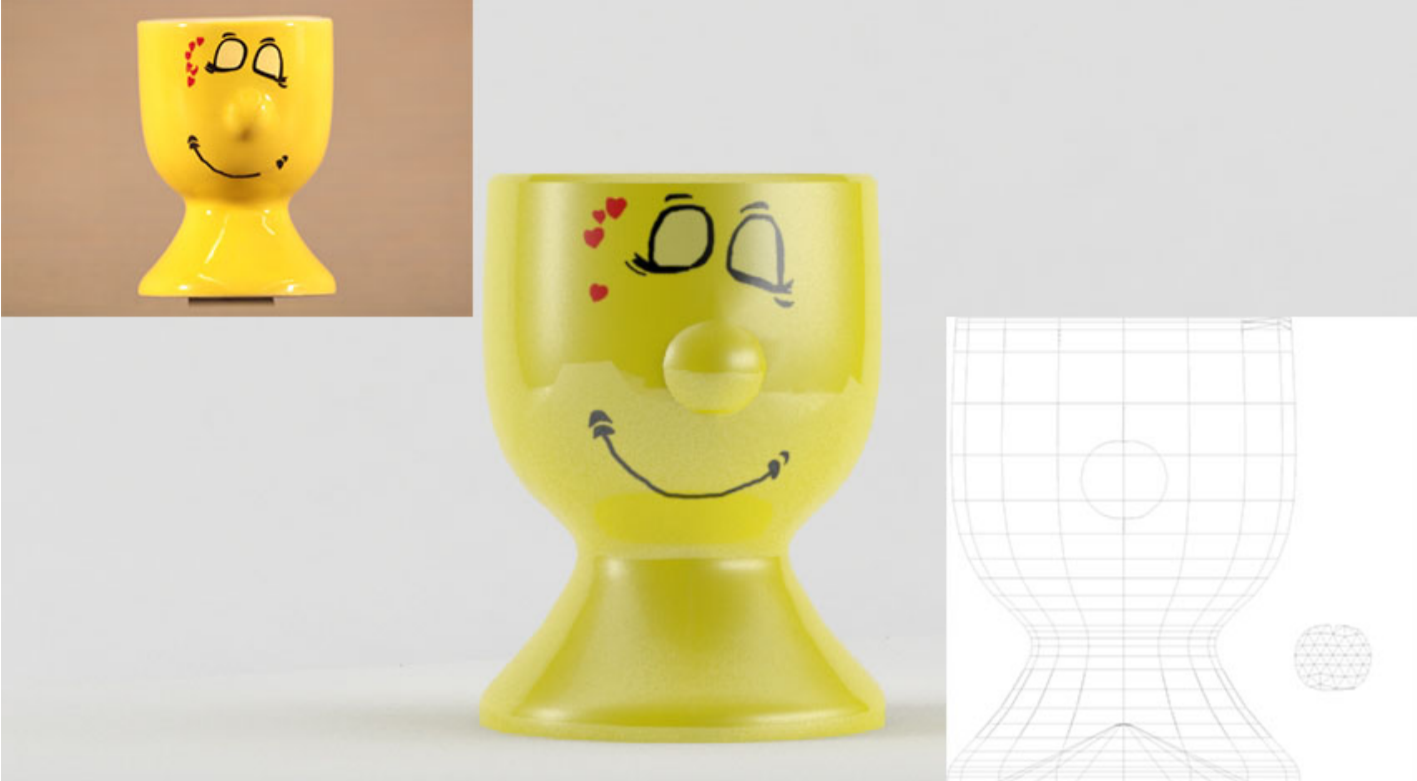
\includegraphics[width=10cm]{img/eggcup.jpg}
		\caption{Simple Egg Cup with UVW Mapped material}
	\label{fig:Egg Cup}
\end{figure}

Upload your model to Moodle upon completion.

\textbf{Late Submission}\\
Failure to submit your assignment on or before the date and time indicated on Moodle will result in a penalty of 5\% per day or part thereof.

\end{document}